\documentclass[11pt]{article}
\usepackage[a4paper,margin=27mm,top=28mm,bottom=30mm]{geometry}
\usepackage[T1]{fontenc}
\usepackage[utf8]{inputenc}
\usepackage{mathpazo}
\usepackage[scaled=0.92]{helvet}
\usepackage{microtype}
\usepackage{amsmath,amssymb,amsthm,mathtools}
\usepackage{booktabs,array,tabularx}
\usepackage{enumitem}
\usepackage{tikz}
\usetikzlibrary{calc,arrows.meta,positioning}
\usepackage{aliascnt}
\usepackage[colorlinks=true,linkcolor=black!70!blue,citecolor=black!60!blue,urlcolor=black!60!blue]{hyperref}
\usepackage[capitalise,noabbrev]{cleveref}
\usepackage{caption}
\captionsetup{font=small,labelfont=bf,width=0.92\textwidth}
\setlist{itemsep=2pt,topsep=3pt}
\linespread{1.04}
\theoremstyle{plain}
\newtheorem{theorem}{Theorem}[section]
% Each environment shares the theorem counter through an alias, so that cleveref names it by its own type.
\newcommand{\sharedthm}[2]{\newaliascnt{#1}{theorem}\newtheorem{#1}[#1]{#2}\aliascntresetthe{#1}\crefname{#1}{#2}{#2s}}
\sharedthm{proposition}{Proposition}
\sharedthm{lemma}{Lemma}
\sharedthm{corollary}{Corollary}
\theoremstyle{definition}
\sharedthm{definition}{Definition}
\sharedthm{question}{Question}
\theoremstyle{remark}
\sharedthm{remark}{Remark}
\newtheorem*{mainA}{Theorem A}
\newtheorem*{mainB}{Theorem B}
\newtheorem*{mainC}{Theorem C}
\newtheorem*{mainD}{Corollary D}
\newcommand{\N}{\mathbb N}
\newcommand{\Q}{\mathbb Q}
\newcommand{\ind}{\mathbf 1}
\newcommand{\eps}{\varepsilon}
\newcommand{\yes}{\mathsf{yes}}
\newcommand{\no}{\mathsf{no}}
\newcommand{\jt}{\mathsf{j}}
\newcommand{\spl}{\mathsf{s}}
\newcommand{\dead}{\dagger}
\newcommand{\start}{\mathsf{start}}
\newcommand{\halt}{\mathsf{halt}}
\newcommand{\gen}{\mathsf{gen}}
\newcommand{\init}{\mathsf{init}}
\newcommand{\un}{\mathtt{u}}
\newcommand{\fin}{\dashv}
\newcommand{\enc}[1]{\langle #1\rangle}
\newcommand{\st}[1]{\ulcorner #1\urcorner}
\newcommand{\src}{\operatorname{src}}
\newcommand{\dst}{\operatorname{dst}}
\newcommand{\out}{\operatorname{out}}
\newcommand{\cert}{\operatorname{cert}}
\newcommand{\acc}{\operatorname{acc}}
\newcommand{\rej}{\operatorname{rej}}
\newcommand{\code}{\operatorname{code}}
\newcommand{\PUSH}{\mathrm{PUSH}}
\newcommand{\POP}{\mathrm{POP}}
\newcommand{\pin}{p_{\circ}}
\newcommand{\perr}{p_{\mathrm{err}}}
\newcommand{\cS}{\mathcal C}
\newcommand{\cI}{\mathcal I}
\newcommand{\cE}{\mathcal E}
\hypersetup{pdftitle={The values of rational probabilistic finite automata are the left-c.e. reals},pdfauthor={Seth Douglas and Nidhal Mghirbi}}
\title{\vspace{-1.2cm}\LARGE The values of rational probabilistic finite automata\\ are the left-c.e.\ reals}
\author{Seth Douglas \and Nidhal Mghirbi}
\date{\small Version 1.0.2, November 2026}
\begin{document}
\maketitle
\begin{abstract}
\noindent
Which real numbers are values of probabilistic finite automata with rational transition probabilities and a rational initial distribution? We show that they are exactly the left-c.e.\ reals in $[0,1]$, the limits of computable nondecreasing sequences of rational numbers. Here the value of an automaton is the supremum, over all finite input words, of the probability that the word is accepted. Every value is left-c.e.\ because the words can be enumerated; we prove that every left-c.e.\ real in $[0,1]$ occurs, and that two input letters and one fixed number of states suffice for all of them.

In particular a single automaton can have a noncomputable value. It was known that no algorithm computes, or even approximates, the value from the automaton; that concerns the map from automata to values, not single values. We give an automaton, specified explicitly relative to a fixed enumeration of Turing machines, whose value is $1/4$ plus the sum of $4^{-(n+2)}$ over the programs $n$ that halt on input $n$. The automaton checks claimed runs of a counter machine by a likelihood test in the manner of Condon and Lipton, and pays out a reward read from each run's output. The construction uses a rational interval around the target; from the target's approximations alone no algorithm can produce the automaton, since an automaton of value $0$ can be recognized. The halting probability of every prefix-free machine, Chaitin's $\Omega$ among them, is the value of a probabilistic finite automaton with two input letters. With a construction of Elkouss and P\'erez-Garc\'ia, every left-c.e.\ real in $[0,1]$ is also the capacity of a finite-state channel with rational transition probabilities; in particular one such channel has a noncomputable capacity.
\end{abstract}
\begin{center}\small AI systems assisted with this work; see ``How this work was done.''\end{center}
{\small\tableofcontents}

\section{Introduction}\label{sec:intro}

A probabilistic finite automaton, introduced by Rabin \cite{Rab63}, has finitely many states. On each input letter it moves from its current state to a random next state, with probabilities given by a stochastic matrix for that letter, and it accepts a word if it ends in an accepting state. We consider automata whose transition probabilities and initial distribution are rational. The \emph{value} $V(A)$ of such an automaton $A$ is the supremum, over all finite words $w$, of the probability $P_A(w)$ that $A$ accepts $w$. Which real numbers are values?

A real number is \emph{left-c.e.}\ if it is the limit of a computable nondecreasing sequence of rational numbers \cite{DH10}. Every value is left-c.e.: each $P_A(w)$ is a rational number computable from $A$ and $w$, and the maximum of $P_A$ over the first $n$ words of an enumeration increases to $V(A)$ (\cref{prop:easy}). This observation is folklore; it amounts to the semi-decidability of the strict emptiness problem, whether $V(A)>\lambda$ for a given rational $\lambda$. Our main result is the converse.

\begin{mainA}
The values of rational probabilistic finite automata are exactly the left-c.e.\ reals in $[0,1]$.
\end{mainA}

\begin{mainB}
There is a number $N$ such that every left-c.e.\ real in $[0,1]$ is the value of a rational probabilistic finite automaton with two input letters and at most $N$ states.
\end{mainB}

The number $N$ is fixed by one universal counter program (\cref{sec:binary}); we have not computed it, and it is large. Two states do not suffice: an automaton with two states has a rational value (\cref{prop:two}).

It has long been known that the value cannot be computed from the automaton. Strict emptiness is undecidable \cite{NH69,Paz71}; the value cannot be approximated to within any fixed error smaller than $1/2$ \cite{CL89,MHC03}; and whether $V(A)=1$ is undecidable \cite{GO10}. Fijalkow derives these results from one theorem \cite{Fij17}. They are statements about the map $A\mapsto V(A)$, and they are compatible with every single value being a computable real, in the same way that equality to $0$ is undecidable for computable reals although each real in question is computable. The remark of Fijalkow, Gimbert, Kelmendi and Oualhadj that, as a consequence of Paz's undecidability result, ``the value of an automaton is not computable in general'' \cite{FGKO15} refers to this map. Rote proved that strict emptiness is undecidable even for one fixed automaton whose initial distribution, or whose vector of final weights, is the input \cite{Rot24,Rot25}; the input there is not the threshold, and his theorem does not show that the value of one automaton is noncomputable. For channels, Boche, Schaefer and Poor treat a single computable finite-state channel with a noncomputable capacity as a stronger, hypothetical form of non-computability, and cite examples for compound and averaged channels with countably infinite sets of states \cite[Remark~31]{BSP20}. For probabilistic finite automata, Theorem~C below gives one automaton with a noncomputable value, and Theorem~A shows that every left-c.e.\ real occurs; through the channels of Elkouss and P\'erez-Garc\'ia \cite{EPG18}, the same holds for capacities of finite-state channels with rational transition probabilities (\cref{cor:channel}).

\begin{mainC}
Fix an effective enumeration of Turing machines. Let $H$ be the set of numbers $n$ such that the $n$-th machine halts on input $n$, and let $\alpha_*=1/4+\sum_{n\in H}4^{-(n+2)}$. Then $\alpha_*$ is not computable, and it is the value of the rational probabilistic finite automaton $A_*$ of \cref{sec:example}, built with the constants $a=1/8$, $b=1/2$ and $B=16$.
\end{mainC}

In particular, for the one automaton $A_*$, the strict emptiness problem with the threshold as the only input is undecidable. Once an effective enumeration of Turing machines is fixed, the automaton $A_*$ is obtained from a specified Turing machine by the compilation of \cref{sec:counter,sec:check,sec:race}; its matrices are large, and we do not list them. Reals defined in this way from a computably enumerable undecidable set go back to Specker \cite{Spe49}.

\begin{mainD}
The halting probability of every prefix-free machine, in particular Chaitin's halting probability $\Omega$ of a universal prefix-free machine, is the value of a rational probabilistic finite automaton with two input letters and at most $N$ states.
\end{mainD}

It is well known that every left-c.e.\ real in $[0,1]$ is the halting probability of some prefix-free machine \cite{CHKW01,DH10}, so Theorem~A says that the values of rational probabilistic finite automata are exactly the halting probabilities of prefix-free machines (\cref{rem:halting}).

The construction is effective once a rational interval $a<\alpha<b$ around the target is given, and it cannot be made effective from a left-c.e.\ index of the target alone: whether $V(A)=0$ can be decided from $A$, while whether a left-c.e.\ real given by an approximating sequence is positive cannot (\cref{prop:uniform}).

Theorem~A has the shape of the theorem of Hochman and Meyerovitch that the topological entropies of shifts of finite type on $\mathbb Z^d$, $d\ge2$, are exactly the nonnegative right-c.e.\ reals \cite{HM10}. In both cases a quantity attached to a finite description has an evident one-sided approximation, from above for entropy and from below for the value of an automaton, and every real with such an approximation occurs. We use this only as an analogy; the methods are different.

\subsection{How the automaton works}

Fix a left-c.e.\ real $\alpha\in(0,1)$ and rationals $0<a<\alpha<b<1$. For a binary word $s=s_1\cdots s_k$ let $x(s)=\sum_{i=1}^k s_i2^{i-k-1}$, the binary fraction $0.s_ks_{k-1}\cdots s_1$, and let $q(s)=a+(b-a)x(s)$. The set $W_\alpha$ of words $s$ with $q(s)<\alpha$ is computably enumerable, so some counter program outputs exactly the words of $W_\alpha$ along its halting runs (\cref{sec:counter}). The input of the automaton is meant to be a sequence of \emph{certificates}, each listing a run of this program: its instructions in order, and the counter values in unary (\cref{fig:mechanism}). A deterministic part of the automaton checks everything except the counter arithmetic. The arithmetic, which a finite automaton cannot check, is tested at random. At the start of each certificate the automaton picks one of two tests with equal probability. The \emph{joint} test survives each unary symbol of both sides of every claimed equation with probability $1/B$; the \emph{split} test picks one side of each equation at random and survives each of its symbols with probability $1/B^2$. On a correct run the two tests survive with the same probability. If any equation is false, the split test is at least $\kappa_B=(B+B^{-1})/2$ times as likely to survive (\cref{lem:test,lem:dichotomy}). Independently, a two-state register holds $x(s)$, for the output $s$ of the claimed run, as the probability of one of its states. At the end of a certificate, a surviving joint test accepts with probability $q(s)$, a surviving split test rejects with probability $1-q(s)$, and all other probability starts afresh. Acceptance and rejection are permanent.

Of the probability that a certificate settles, a correct certificate therefore accepts the fraction $q(s)<\alpha$, and an incorrect one a fraction at most $b/(b+\kappa_B(1-b))$, which is below $a$ once $B$ is large. Every input word, however it mixes correct, incorrect and malformed certificates, is accepted with probability at most $\alpha$. Repeating one correct certificate drives the acceptance probability up to $q(s)$, and these rewards approach $\alpha$.

\begin{figure}[t]
\centering
\resizebox{0.86\textwidth}{!}{%
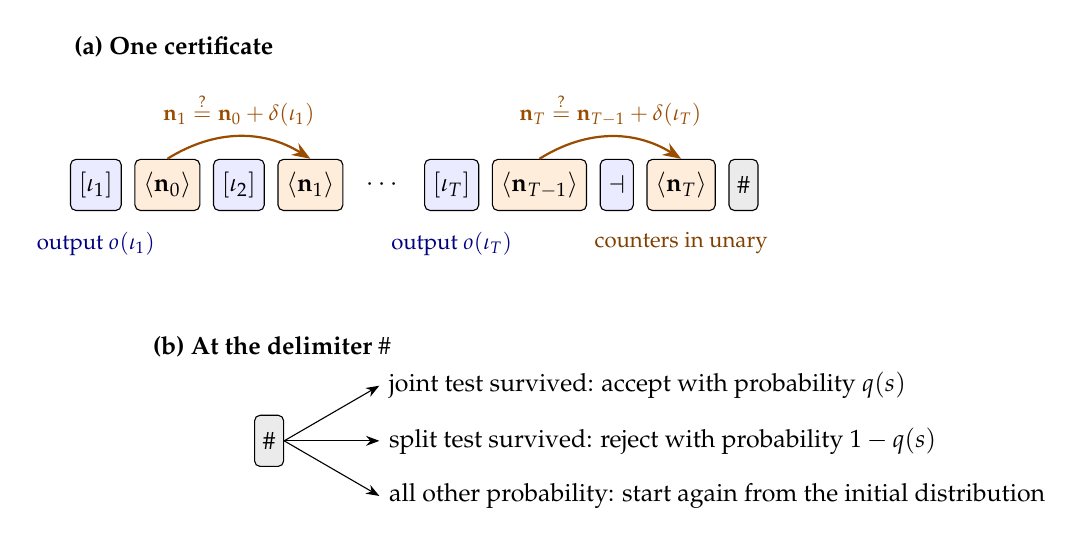
\begin{tikzpicture}[font=\small,>=Stealth,
 box/.style={draw,rounded corners=2pt,minimum height=6.5mm,inner sep=3pt},
 ins/.style={box,fill=blue!8},
 cnt/.style={box,fill=orange!14},
 node distance=1.6mm]
\node[font=\small\bfseries,anchor=west] at (-0.4,1.75) {(a) One certificate};
\node[ins] (i1) at (0,0) {$[\iota_1]$};
\node[cnt,right=of i1] (c0) {$\enc{\mathbf n_0}$};
\node[ins,right=of c0] (i2) {$[\iota_2]$};
\node[cnt,right=of i2] (c1) {$\enc{\mathbf n_1}$};
\node[right=of c1] (dots) {$\cdots$};
\node[ins,right=of dots] (iT) {$[\iota_T]$};
\node[cnt,right=of iT] (cT1) {$\enc{\mathbf n_{T-1}}$};
\node[ins,right=of cT1] (fin) {$\fin$};
\node[cnt,right=of fin] (cT) {$\enc{\mathbf n_T}$};
\node[box,fill=black!8,right=of cT] (h) {$\#$};
\draw[->,thick,orange!60!black] (c0.north) to[bend left=32] node[above,font=\footnotesize]{$\mathbf n_1\overset{?}{=}\mathbf n_0+\delta(\iota_1)$} (c1.north);
\draw[->,thick,orange!60!black] (cT1.north) to[bend left=32] node[above,font=\footnotesize]{$\mathbf n_T\overset{?}{=}\mathbf n_{T-1}+\delta(\iota_T)$} (cT.north);
\node[below=1.5mm of i1,font=\footnotesize,blue!50!black,anchor=north] {output $o(\iota_1)$};
\node[below=1.5mm of iT,font=\footnotesize,blue!50!black,anchor=north] {output $o(\iota_T)$};
\node[below=1.5mm of cT,font=\footnotesize,orange!50!black,anchor=north] {counters in unary};
\begin{scope}[shift={(2.2,-2.3)}]
\node[font=\small\bfseries,anchor=west] at (-1.6,0.25) {(b) At the delimiter $\#$};
\node[box,fill=black!8] (hh) at (0,-0.95) {$\#$};
\node[anchor=west] (r1) at (1.4,-0.25) {joint test survived: accept with probability $q(s)$};
\node[anchor=west] (r2) at (1.4,-0.95) {split test survived: reject with probability $1-q(s)$};
\node[anchor=west] (r3) at (1.4,-1.65) {all other probability: start again from the initial distribution};
\draw[->] (hh.east) -- (r1.west);
\draw[->] (hh.east) -- (r2.west);
\draw[->] (hh.east) -- (r3.west);
\end{scope}
\end{tikzpicture}}
\caption{(a) A certificate lists a claimed run of a counter program. Each row is the next instruction, or $\fin$ for the last row, followed by the counter values in unary. A deterministic parser checks everything except the equations between consecutive rows, which are tested at random. (b) At the delimiter a surviving joint test accepts with probability $q(s)$ and a surviving split test rejects with probability $1-q(s)$, where $s$ is the output listed in the certificate; everything else starts again. Acceptance and rejection are permanent.}
\label{fig:mechanism}
\end{figure}

\subsection{Prior work}

\Cref{tab:landscape} lists what was known about the value and what is proved here. The verification of counter-machine runs by a probabilistic finite automaton, through coin-flipping comparisons of unary lengths, is due to Condon and Lipton \cite{CL89}, who used an equality test of Freivalds \cite{Fre81} to prove that emptiness is undecidable with a gap; Madani, Hanks and Condon \cite{MHC99,MHC03} and Rote \cite{Rot24} give detailed accounts. Our joint and split tests are a form of this test. What we add is the payout at the delimiter: the surviving tests accept and reject in proportions set by a reward read from the certificate's output, so that the value of the automaton is the supremum of the rewards rather than one of two values separated by a gap. For partially observable Markov decision processes the value is likewise known to be uncomputable as a function of the process \cite{MHC03}; \cref{prop:pomdp} records the range of values for reachability objectives.

\begin{table}[t]
\centering\small
\begin{tabularx}{\textwidth}{@{}>{\raggedright\arraybackslash}X >{\raggedright\arraybackslash}p{0.22\textwidth} >{\raggedright\arraybackslash}p{0.2\textwidth}@{}}
\toprule
Statement & Scope & Source\\
\midrule
Every value is left-c.e. & every automaton & folklore\\[3pt]
Whether $V(A)>\lambda$ is undecidable & uniform in $A,\lambda$ & \cite{NH69,Paz71}\\[3pt]
$V(A)$ cannot be approximated to within any fixed error below $1/2$ & uniform in $A$ & \cite{CL89,MHC03,Fij17}\\[3pt]
Whether $V(A)=1$ is undecidable & uniform in $A$ & \cite{GO10}\\[3pt]
Emptiness is undecidable for one fixed set of matrices, with the initial distribution or the final vector as input & one set of matrices, varying vectors & \cite{Rot24,Rot25}\\[3pt]
One automaton has a noncomputable value & one automaton & Theorem~C\\[3pt]
The values are exactly the left-c.e.\ reals in $[0,1]$ & every left-c.e.\ real & Theorem~A\\[3pt]
Two letters and at most $N$ states realize every value & one bound for all values & Theorem~B\\[3pt]
Every prefix-free halting probability is a value & every halting probability & Corollary~D\\
\bottomrule
\end{tabularx}
\caption{What was known about the value $V(A)$ of a rational probabilistic finite automaton, and what is proved here.}
\label{tab:landscape}
\end{table}

\paragraph{Reading guide.} \Cref{sec:prelim} fixes definitions and proves the easy inclusion. \Cref{sec:counter} constructs counter programs that output a given computably enumerable set of words; it is Minsky's simulation of Turing machines with outputs added, and a reader who knows it can take \cref{lem:program,lem:universal} as given. \Cref{sec:check} builds the random check of one certificate, and \cref{sec:race} adds the payout and proves Theorem~A. \Cref{sec:example} proves Theorem~C and Corollary~D, the latter using Theorem~B, which \cref{sec:binary} proves; and \cref{sec:uniform} discusses uniformity. \Cref{sec:open} collects open problems, with two classes of automata whose values are computable and the corresponding statement for partially observable Markov decision processes.

\section{Preliminaries}\label{sec:prelim}

\begin{definition}\label{def:pfa}
A \emph{rational probabilistic finite automaton} is a tuple $A=(Q,\Sigma,(M_\ell)_{\ell\in\Sigma},\pi,F)$, where $Q$ and $\Sigma$ are finite nonempty sets, each $M_\ell$ is a row-stochastic $Q\times Q$ matrix with rational entries, $\pi$ is a probability row vector on $Q$ with rational entries, and $F\subseteq Q$. For a word $w=\ell_1\cdots\ell_k$ over $\Sigma$ let $M_w=M_{\ell_1}\cdots M_{\ell_k}$, with $M_\eps$ the identity, and let $P_A(w)=\pi M_w\ind_F$, where $\ind_F$ is the indicator column of $F$. The \emph{value} of $A$ is $V(A)=\sup_{w\in\Sigma^*}P_A(w)$.
\end{definition}

The empty word is included, so $V(A)\ge\pi\ind_F$. We describe automata by random transition rules: to say that on letter $\ell$ the automaton moves from state $p$ to a random state with a given law means that row $p$ of $M_\ell$ is that law. An automaton made of finitely many components, each with finitely many states, that update by independent random choices has the product of the component state sets as its state set, and the entries of its matrices are products of the probabilities of the components; it is a rational automaton when all these probabilities are rational.

\begin{definition}
A real $\alpha$ is \emph{left-c.e.}\ if $\alpha=\lim_n\alpha_n$ for a computable nondecreasing sequence $(\alpha_n)$ of rationals. An index of a Turing machine that computes $n\mapsto\alpha_n$ is a \emph{left-c.e.\ index} of $\alpha$.
\end{definition}

If $(\alpha_n)$ is such a sequence, a rational $r$ satisfies $r<\alpha$ if and only if $\alpha_n>r$ for some $n$. Hence the set of rationals below $\alpha$ is computably enumerable, uniformly in a left-c.e.\ index of $\alpha$. An \emph{enumeration index} of a computably enumerable set $W$ is an index, in a fixed effective enumeration of Turing machines, of a machine that halts on exactly the elements of $W$.

\begin{proposition}[folklore]\label{prop:easy}
The value of every rational probabilistic finite automaton is a left-c.e.\ real in $[0,1]$.
\end{proposition}

\begin{proof}
Enumerate $\Sigma^*$ as $w_0,w_1,\dots$. The numbers $v_n=\max_{i\le n}P_A(w_i)$ are rationals in $[0,1]$, computable from $n$ by exact arithmetic, nondecreasing, and they converge to $\sup_iP_A(w_i)=V(A)$.
\end{proof}

\section{Counter programs that output words}\label{sec:counter}

\begin{definition}\label{def:program}
A \emph{counter program} $P$ with $d$ counters consists of a finite set $\cS$ of control states with two distinct states $\start$ and $\halt$, and a finite set $\cI$ of instructions. Each instruction $\iota$ has a source $\src(\iota)\in\cS\setminus\{\halt\}$, a destination $\dst(\iota)\in\cS$, a guard $g(\iota)\in\{0,+,*\}^d$, an increment $\delta(\iota)\in\{-1,0,1\}^d$ with $g_j(\iota)={+}$ whenever $\delta_j(\iota)=-1$, and an output $o(\iota)\in\{0,1,\eps\}$. A \emph{configuration} is a pair $(c,\mathbf n)\in\cS\times\N^d$. The instruction $\iota$ is \emph{enabled} at $(c,\mathbf n)$ if $\src(\iota)=c$ and, for every $j$, $n_j=0$ when $g_j(\iota)=0$ and $n_j>0$ when $g_j(\iota)={+}$; it then leads to $(\dst(\iota),\mathbf n+\delta(\iota))$. A \emph{run} from $\mathbf m\in\N^d$ is a sequence $(c_0,\mathbf n_0),\iota_1,(c_1,\mathbf n_1),\dots,\iota_T,(c_T,\mathbf n_T)$ with $(c_0,\mathbf n_0)=(\start,\mathbf m)$ and $c_T=\halt$, in which each $\iota_i$ is enabled at $(c_{i-1},\mathbf n_{i-1})$ and leads to $(c_i,\mathbf n_i)$. Its output is the binary word $o(\iota_1)\cdots o(\iota_T)$, where $\eps$ is the empty word. We write $L(P,\mathbf m)$ for the set of outputs of runs from $\mathbf m$, and $L(P)=L(P,\mathbf 0)$.
\end{definition}

The program may be nondeterministic: several instructions may be enabled at one configuration. We prove two lemmas. The first is Minsky's simulation of Turing machines by counter machines \cite{Min61,Min67}, with a nondeterministic phase that writes the output; the second is its universal version.

\begin{lemma}\label{lem:program}
For every computably enumerable set $W$ of binary words there is a counter program $P$ with three counters such that $L(P)=W$. The program can be computed from an enumeration index of $W$.
\end{lemma}

\begin{lemma}\label{lem:universal}
There are a counter program $U$ with four counters $x_0,x_1,x_2,x_3$ and a sequence $(W_e)_{e\in\N}$ of sets of binary words such that $L(U,(e,0,0,0))=W_e$ for every $e$, and such that for every computably enumerable set $W$ of binary words some $e$, computable from an enumeration index of $W$, satisfies $W_e=W$.
\end{lemma}

\paragraph{Turing machines.} We use deterministic one-tape Turing machines $M$ with a finite set $K$ of states, a start state $k_0$, a halting state $k_h$, a finite tape alphabet $\Gamma$ containing $0$, $1$ and the blank $\square$, and a transition function $\delta_M\colon(K\setminus\{k_h\})\times\Gamma\to K\times\Gamma\times\{-1,0,1\}$. The cells of the tape are indexed by $\mathbb Z$. On input $y=y_0\cdots y_{m-1}$ the machine starts in $k_0$ with $y_i$ in cell $i$, blanks elsewhere, and the head on cell $0$; it \emph{halts} on $y$ if it reaches $k_h$. A set of binary words is computably enumerable if and only if it is the set of binary words on which some such machine halts \cite{Soa16}. For a word $y$ we write $y^R$ for its reversal; the reversal of a computably enumerable set is computably enumerable.

\paragraph{Stacks in counters.} Fix a machine $M$, let $h=|\Gamma|+1$, and fix a bijection $\code\colon\Gamma\to\{1,\dots,h-1\}$. A finite sequence $\gamma_1\gamma_2\cdots\gamma_r$ over $\Gamma$, read as a stack with top $\gamma_1$, is stored in a counter as
\[
\st{\gamma_1\cdots\gamma_r}=\sum_{i=1}^r\code(\gamma_i)\,h^{i-1},
\]
and the empty sequence is stored as $0$. All base-$h$ digits of a stored number are nonzero, so the number determines the sequence. A configuration of $M$ in state $k$, with tape $\tau\colon\mathbb Z\to\Gamma$ and head on cell $z$, is \emph{represented} by the control state $(k,\tau(z))$ together with counter values $x_1=\st{\tau(z-1)\cdots\tau(z-r)}$, $x_2=\st{\tau(z+1)\cdots\tau(z+r')}$ and $x_3=0$, for some $r,r'\ge0$ such that every cell beyond those listed is blank. Different choices of $r,r'$ represent the same configuration.

\begin{lemma}[Stack operations]\label{lem:macros}
Let $i\in\{1,2\}$ and $\gamma\in\Gamma$. There are finite sets of instructions without output, $\PUSH_i(\gamma)$ with an entry state and an exit state, and $\POP_i$ with an entry state and exit states $\mathrm{exit}_{\gamma'}$ for $\gamma'\in\Gamma$, with the following properties. At every control state of these sets other than the exits, exactly one instruction is enabled at each configuration. Started at the entry of $\PUSH_i(\gamma)$ with $x_3=0$ and $x_i$ storing a sequence $\sigma$, the instructions lead to the exit with $x_i$ storing $\gamma\sigma$, $x_3=0$ and the other counters unchanged. Started at the entry of $\POP_i$ with $x_3=0$ and $x_i$ storing $\sigma$, they lead to $\mathrm{exit}_{\gamma'}$, where $\gamma'$ is the top of $\sigma$, or $\square$ if $\sigma$ is empty, with $x_i$ storing $\sigma$ without its top, $x_3=0$ and the other counters unchanged.
\end{lemma}

\begin{proof}
For $\PUSH_i(\gamma)$ use control states $\eta,\eta_1,\dots,\eta_{h-1},\zeta,\zeta_1,\dots,\zeta_{\code(\gamma)}$, with entry $\eta$. At $\eta$: if $x_i>0$, decrement $x_i$, increment $x_3$ and go to $\eta_1$; if $x_i=0$, go to $\zeta$. At $\eta_l$ for $l<h-1$: increment $x_3$ and go to $\eta_{l+1}$; at $\eta_{h-1}$: increment $x_3$ and go to $\eta$. At $\zeta$: if $x_3>0$, decrement $x_3$, increment $x_i$ and stay at $\zeta$; if $x_3=0$, go to $\zeta_1$. At $\zeta_l$ for $l<\code(\gamma)$: increment $x_i$ and go to $\zeta_{l+1}$; at $\zeta_{\code(\gamma)}$: increment $x_i$ and go to the exit. Each pass from $\eta$ back to $\eta$ moves one unit out of $x_i$ and $h$ units into $x_3$, so on reaching $\zeta$ we have $x_i=0$ and $x_3=h\cdot\st\sigma$; the loop at $\zeta$ moves this back, and the chain $\zeta_1,\dots,\zeta_{\code(\gamma)}$ adds $\code(\gamma)$. The result is $h\st\sigma+\code(\gamma)=\st{\gamma\sigma}$.

For $\POP_i$ use control states $\eta_0,\dots,\eta_{h-1}$ and $\zeta_0,\dots,\zeta_{h-1}$, with entry $\eta_0$. At $\eta_l$: if $x_i>0$ and $l<h-1$, decrement $x_i$ and go to $\eta_{l+1}$; if $x_i>0$ and $l=h-1$, decrement $x_i$, increment $x_3$ and go to $\eta_0$; if $x_i=0$, go to $\zeta_l$. At $\zeta_l$: if $x_3>0$, decrement $x_3$, increment $x_i$ and stay at $\zeta_l$; if $x_3=0$, go to $\mathrm{exit}_{\gamma'}$ with $\code(\gamma')=l$ if $l\ge1$, and to $\mathrm{exit}_\square$ if $l=0$. By induction, after $X$ decrements of $x_i$ the program is at $\eta_{X\bmod h}$ with $x_3=\lfloor X/h\rfloor$. Let $X_0=\st\sigma$. If $\sigma$ is empty, $X_0=0$ and the program goes from $\eta_0$ to $\zeta_0$ to $\mathrm{exit}_\square$ with all counters unchanged. Otherwise $X_0=h\st{\sigma'}+\code(\gamma')$, where $\gamma'$ is the top of $\sigma$ and $\sigma'$ the rest, so the decrements end at $\eta_l$ with $l=\code(\gamma')\ge1$ and $x_3=\st{\sigma'}$, and the loop at $\zeta_l$ moves $\st{\sigma'}$ back into $x_i$. In both sets the enabled instruction at each state is unique, because the alternatives have complementary guards.
\end{proof}

\begin{proof}[Proof of \cref{lem:program}]
Let $M$ be a Turing machine that halts on exactly the binary words in $W^R=\{s^R:s\in W\}$. The program $P$ has the counters $x_1,x_2,x_3$, the control states $\start$, $\halt$, the pairs $(k,\gamma)\in K\times\Gamma$, and the states of the copies of the stack operations used below, each copy with its own states. Its instructions are:
\begin{enumerate}[label=(G\arabic*)]
\item for $v\in\{0,1\}$, an instruction from $\start$ with output $v$ to the entry of a copy of $\PUSH_2(v)$ whose exit is $\start$;
\item an instruction from $\start$ to the entry of a copy of $\POP_2$ whose exit $\mathrm{exit}_\gamma$ is $(k_0,\gamma)$ for each $\gamma$;
\end{enumerate}
\begin{enumerate}[label=(S)]
\item for $k\ne k_h$ and $\gamma\in\Gamma$ with $\delta_M(k,\gamma)=(k',\gamma',D)$: if $D=0$, an instruction from $(k,\gamma)$ to $(k',\gamma')$; if $D=+1$, an instruction from $(k,\gamma)$ to a copy of $\PUSH_1(\gamma')$ whose exit is the entry of a copy of $\POP_2$ with exits $(k',\cdot)$; if $D=-1$, the same with $\PUSH_2(\gamma')$ and $\POP_1$;
\end{enumerate}
\begin{enumerate}[label=(H)]
\item for each $\gamma$, an instruction from $(k_h,\gamma)$ to $\halt$.
\end{enumerate}
Only the instructions (G1) have an output. Instructions outside the copies of the stack operations have guard $(*,*,*)$ and increment $0$.

Consider a run from $\mathbf 0$. At $\start$ the run uses (G1) some number $m\ge0$ of times, with bits $s_1,\dots,s_m$, each followed by its copy of $\PUSH_2$, and then (G2). By \cref{lem:macros}, before (G2) we have $x_1=x_3=0$ and $x_2=\st{s_m s_{m-1}\cdots s_1}$, and after the copy of $\POP_2$ the control state is $(k_0,\gamma)$ with $\gamma=s_m$, or $\gamma=\square$ if $m=0$, and $x_2=\st{s_{m-1}\cdots s_1}$. This represents the start of $M$ on the input $s_m\cdots s_1=s^R$, where $s=s_1\cdots s_m$. From then on exactly one instruction is enabled at each configuration, and by \cref{lem:macros} a pass through one instruction (S) and its copies maps a representation of a configuration of $M$ to a representation of the next configuration: for $D=+1$, pushing $\gamma'$ onto $x_1$ lists the cells to the left of the new head position, and popping $x_2$ yields the symbol under it, or a blank. Hence the run reaches $\halt$ if and only if $M$ halts on $s^R$, that is, if and only if $s\in W$. Its output is $s$, because only (G1) has an output. Conversely, for each $s\in W$ the choices above give a run with output $s$. So $L(P)=W$. Every step is effective in $M$, and $M$ is computable from an enumeration index of $W$.
\end{proof}

\begin{proof}[Proof of \cref{lem:universal}]
Fix an effective enumeration $(M_e)_{e\in\N}$ of the Turing machines above. By the existence of a universal Turing machine, which goes back to Turing \cite{Tur36} (for the formulation with halting used here see, for example, \cite{Min67,Soa16}), there is one Turing machine $T_U$, whose tape alphabet contains a symbol $\sharp$, such that for all $e\in\N$ and all binary words $y$, $T_U$ halts on the input $1^e\sharp y$ if and only if $M_e$ halts on $y$. Let $W_e=\{s:M_e\text{ halts on }s^R\}$. If $W$ is computably enumerable, so is $W^R$, and any $e$ such that $M_e$ halts on exactly the binary words in $W^R$ satisfies $W_e=W$; such an $e$ is computable from an index of $W$.

The program $U$ has the counters $x_0,\dots,x_3$, where $x_0$ is only used as described now, and the instructions (G1), (S) and (H) of the proof of \cref{lem:program}, with $T_U$ in place of $M$. Instead of (G2) it has an instruction from $\start$ to a copy of $\PUSH_2(\sharp)$ whose exit is a new control state $\init$, and at $\init$: if $x_0>0$, an instruction that decrements $x_0$ and goes to a copy of $\PUSH_2(1)$ whose exit is $\init$; if $x_0=0$, an instruction to a copy of $\POP_2$ with exits $(k_0,\cdot)$. A run from $(e,0,0,0)$ with output $s=s_1\cdots s_m$ reaches $\init$ with $x_2=\st{\sharp s_m\cdots s_1}$, leaves it with $x_0=0$ and $x_2=\st{1^e\sharp s_m\cdots s_1}$, and after the copy of $\POP_2$ represents the start of $T_U$ on $1^e\sharp s^R$. As before, the run reaches $\halt$ if and only if $T_U$ halts on $1^e\sharp s^R$, that is, if and only if $s\in W_e$. The instructions of $U$ do not depend on $e$.
\end{proof}

\section{Checking a run with two random tests}\label{sec:check}

\subsection{The equality test}

\begin{lemma}\label{lem:test}
Let $B\ge2$ be an integer and $\kappa_B=(B+B^{-1})/2$. For $n,n'\in\N$ put
\[
\varphi_B(n,n')=B^{-(n+n')},\qquad \psi_B(n,n')=\tfrac12\bigl(B^{-2n}+B^{-2n'}\bigr).
\]
Then $\psi_B(n,n')=\varphi_B(n,n')$ if $n=n'$, and $\psi_B(n,n')\ge\kappa_B\,\varphi_B(n,n')$ if $n\ne n'$.
\end{lemma}

\begin{proof}
The ratio is $\psi_B/\varphi_B=g(n-n')$ with $g(t)=(B^t+B^{-t})/2$. The function $g$ is even, $g(0)=1$, and for integers $t\ge0$
\[
g(t+1)-g(t)=\tfrac12(B-1)\bigl(B^t-B^{-t-1}\bigr)>0 .
\]
Hence $g(t)\ge g(1)=\kappa_B$ for every integer $t\ne0$.
\end{proof}

A finite automaton realizes $\varphi_B$ by surviving each unary symbol of both lengths with probability $1/B$, and $\psi_B$ by choosing one of the two lengths with a fair coin and surviving each of its symbols with probability $1/B^2$. Since $\kappa_B\to\infty$, a single false equation makes the second experiment much more likely to survive than the first.

\subsection{Certificates}

Fix a counter program $P$ with $d$ counters. Its certificate alphabet is
\[
\Sigma_P=\{[\iota]:\iota\in\cI\}\cup\{\fin,\un,\diamond,\#\}.
\]
For $\mathbf n\in\N^d$ let $\enc{\mathbf n}=\un^{n_1}\diamond\un^{n_2}\diamond\cdots\un^{n_d}\diamond$, the $d$ \emph{blocks} of $\mathbf n$.

\begin{definition}\label{def:certificate}
A \emph{certificate} is a word
\[
t=[\iota_1]\enc{\mathbf n_0}[\iota_2]\enc{\mathbf n_1}\cdots[\iota_T]\enc{\mathbf n_{T-1}}\fin\enc{\mathbf n_T}\#
\]
with $T\ge0$, $\iota_i\in\cI$ and $\mathbf n_i\in\N^d$. Its \emph{rows} are the words $[\iota_{i+1}]\enc{\mathbf n_i}$ for $i<T$ and $\fin\enc{\mathbf n_T}$; row $i$ has the \emph{head} $[\iota_{i+1}]$ or $\fin$. Its \emph{output} is $\out(t)=o(\iota_1)\cdots o(\iota_T)$. It is \emph{well formed} if
\begin{enumerate}[label=(W\arabic*)]
\item $T\ge1$, $\src(\iota_1)=\start$, $\src(\iota_{i+1})=\dst(\iota_i)$ for $1\le i<T$, and $\dst(\iota_T)=\halt$;
\item $\mathbf n_0=\mathbf 0$;
\item for $0\le i<T$, the vector $\mathbf n_i$ satisfies the guard of $\iota_{i+1}$.
\end{enumerate}
Its \emph{equations} are the pairs, for $0\le i<T$ and $1\le j\le d$,
\[
E_{i,j}=\bigl(n_{i,j}+\delta^+,\;n_{i+1,j}+\delta^-\bigr),\qquad \delta=\delta_j(\iota_{i+1}),
\]
where $\delta^+=\max(\delta,0)$ and $\delta^-=\max(-\delta,0)$; the two numbers are its \emph{members}. A well-formed certificate is \emph{valid} if the two members of every equation are equal.
\end{definition}

The members of $E_{i,j}$ are equal if and only if $n_{i+1,j}=n_{i,j}+\delta_j(\iota_{i+1})$. To a run $\rho$ from $\mathbf 0$ as in \cref{def:program} we associate the certificate $\cert(\rho)=[\iota_1]\enc{\mathbf n_0}\cdots[\iota_T]\enc{\mathbf n_{T-1}}\fin\enc{\mathbf n_T}\#$.

\begin{lemma}\label{lem:valid}
A certificate is valid if and only if it is $\cert(\rho)$ for a run $\rho$ of $P$ from $\mathbf 0$, and then its output is the output of $\rho$.
\end{lemma}

\begin{proof}
Put $c_0=\start$ and $c_i=\dst(\iota_i)$. Conditions (W1)--(W3) and the equalities $\mathbf n_{i+1}=\mathbf n_i+\delta(\iota_{i+1})$ say exactly that $(c_0,\mathbf n_0),\iota_1,\dots,\iota_T,(c_T,\mathbf n_T)$ is a run from $\mathbf 0$. The outputs agree by definition.
\end{proof}

\subsection{The parser}

\begin{lemma}\label{lem:parser}
There is a deterministic finite automaton over $\Sigma_P$, the \emph{parser}, with an initial state $\pin$ and an absorbing error state $\perr$, such that for every word $w$ the parser started in $\pin$ is in $\pin$ after reading $w$ if and only if $w$ is a concatenation of well-formed certificates, and it does not enter $\perr$ while it reads a prefix of such a concatenation. While it reads a letter $\un$ or $\diamond$, its state determines the head of the current row, the index $j$ of the current block, and whether the current row is row~$0$.
\end{lemma}

\begin{proof}
A state of the parser outside $\{\pin,\perr\}$ records the control state $c$ that the next head must have as its source, the head of the current row, the index $j\in\{1,\dots,d+1\}$ of the current block ($d+1$ once the row is complete), whether the current block has a symbol $\un$ yet, and whether the current row is row~$0$. In $\pin$ the expected source is $\start$, no row has started, and the next row is row~$0$. On a head $[\iota]$ at the start of a row, the parser checks $\src(\iota)=c$, records $\iota$ and sets $c=\dst(\iota)$. On $\fin$ at the start of a row it checks $c=\halt$, which excludes $T=0$ because $\start\ne\halt$, and then replaces $c$ by a mark that is the source of no instruction and is not $\halt$; so after a row with head $\fin$ is complete, the only allowed letter is $\#$. On $\un$ it checks that the current row is not row~$0$ and that the guard of the head does not require the current counter to be zero; for these checks the head $\fin$ of a final row counts as having a guard with no requirements. On $\diamond$ it checks that the guard does not require the current counter to be positive when the block is empty, and moves to the next block. On $\#$ it checks that the current row is complete and has head $\fin$, and returns to $\pin$. Every other letter, for instance $\un$ or $\diamond$ after the last block of a row, and every failed check, leads to $\perr$. These checks are exactly (W1)--(W3) and the format of \cref{def:certificate}, and each is made at the letter that completes the condition checked, so a prefix of a concatenation of well-formed certificates passes all of them.
\end{proof}

\subsection{The checking automaton}

Fix $P$ and an integer $B\ge2$. The checking automaton has the following states. A \emph{live} state is either $(p,\jt,r)$ or $(p,\spl,\xi,r)$, where $p\ne\perr$ is a parser state, $\jt$ and $\spl$ mark the joint and the split test, $r\in\{0,1\}$ is the \emph{register}, and $\xi=(\xi^{\mathrm{in}}_j,\xi^{\mathrm{out}}_j)_{j\le d}$ with entries in $\{\emptyset,1,2\}$ records the choices of the split test. A \emph{dead} state is $(p,\dead)$ with $p\ne\perr$. There are two further states, $\yes$ and $\no$. The initial distribution $\pi_\circ$ gives probability $1/2$ to $(\pin,\jt,0)$ and $1/2$ to $(\pin,\spl,\emptyset,0)$, where $\emptyset$ denotes the vector with all entries $\emptyset$.

In a block $j$ of row $i$, let $\chi_j\in\{0,1,2\}$ be the number of equations of which this block is a member: $\chi_j=[i\ge1]+[\text{the head of row $i$ is not $\fin$}]$. By \cref{lem:parser} the parser state determines $\chi_j$. For a letter $\ell\ne\#$, let $p'$ be the parser state after $\ell$, and let $o(\ell)=o(\iota)$ if $\ell=[\iota]$ and $o(\ell)=\eps$ otherwise. The two-state register matrices are
\[
R_0=\begin{pmatrix}1&0\\ 1/2&1/2\end{pmatrix},\qquad R_1=\begin{pmatrix}1/2&1/2\\ 0&1\end{pmatrix},\qquad R_\eps=\begin{pmatrix}1&0\\0&1\end{pmatrix},
\]
in the state order $0,1$. On $\ell\ne\#$ the checking automaton acts as follows.
\begin{enumerate}[label=(C\arabic*)]
\item If $p'=\perr$, every live or dead state moves to $\no$.
\item Otherwise a dead state $(p,\dead)$ moves to $(p',\dead)$. A live state moves its parser state to $p'$ and its register from $r$ to $r'$ with probability $R_{o(\ell)}(r,r')$, independently of everything else, and it survives with the probability given below; if it does not survive it moves to $(p',\dead)$.
\item Joint test. On $[\iota]$ it survives with probability $B^{-\sum_j|\delta_j(\iota)|}$; on $\un$ in block $j$ with probability $B^{-\chi_j}$; on other letters with probability $1$.
\item Split test. On $[\iota]$ it draws $\xi^{\mathrm{out}}_j\in\{1,2\}$ uniformly and independently for $j=1,\dots,d$, and survives with probability
\[
\prod_{j=1}^dB^{-2\left(\delta_j^+[\xi^{\mathrm{out}}_j=1]+\delta_j^-[\xi^{\mathrm{out}}_j=2]\right)},\qquad \delta_j=\delta_j(\iota).
\]
On $\un$ in block $j$ it survives with probability $B^{-2([\xi^{\mathrm{in}}_j=2]+[\xi^{\mathrm{out}}_j=1])}$. On the separator $\diamond$ that closes block $j$ it survives with probability $1$ and replaces $(\xi^{\mathrm{in}}_j,\xi^{\mathrm{out}}_j)$ by $(\xi^{\mathrm{out}}_j,\emptyset)$. On other letters it survives with probability $1$ and keeps $\xi$.
\end{enumerate}
Here $[\cdot]$ is $1$ if the condition holds and $0$ otherwise. The choice $\xi^{\mathrm{out}}_j$ drawn at the head of row $i$ is the choice of the split test for the equation $E_{i,j}$: the value $1$ selects its first member and $2$ its second. It is kept in $\xi^{\mathrm{out}}_j$ while block $j$ of row $i$ is read, then in $\xi^{\mathrm{in}}_j$ while block $j$ of row $i+1$ is read, and then discarded. At each moment at most two equations per counter have a recorded choice, so the state set is finite. All probabilities are rational, and each row sums to $1$. The rows of $\yes$ and $\no$, and the action of $\#$, are given in \cref{sec:race}.

For a well-formed certificate $t=t'\#$ with equations $\cE(t)=\{E_{i,j}\}$, put
\[
\Phi(t)=\frac12\prod_{(n,n')\in\cE(t)}\varphi_B(n,n'),\qquad \Psi(t)=\frac12\prod_{(n,n')\in\cE(t)}\psi_B(n,n').
\]
For a binary word $s=s_1\cdots s_k$ let $x(s)=\sum_{i=1}^ks_i2^{i-k-1}$, so that $x(\eps)=0$ and $x(sv)=(x(s)+v)/2$ for a bit $v$.

\begin{lemma}\label{lem:masses}
Let $t=t'\#$ be a well-formed certificate with output $s$. Started from $\pi_\circ$, after reading $t'$ the checking automaton is in live joint states with total probability $\Phi(t)$, in live split states with total probability $\Psi(t)$, and in dead states otherwise. Within each of the two live parts, the register is $1$ with conditional probability $x(s)$.
\end{lemma}

\begin{proof}
No letter of $t'$ leads the parser to $\perr$, so (C1) does not occur, and the parser state is the same for all states at every moment.

Joint test. Its survival probability is the product of the factors in (C3). A symbol $\un$ in block $j$ of row $i$ contributes $B^{-1}$ for each equation of which the block is a member, and the head $[\iota_{i+1}]$ contributes $B^{-1}$ for each unit of the offsets $\delta^+$ and $\delta^-$ in the equations $E_{i,j}$, since $\delta^++\delta^-=|\delta|$. The product is therefore $\prod_{(n,n')\in\cE(t)}B^{-(n+n')}$, and with the initial factor $1/2$ the probability is $\Phi(t)$.

Split test. Fix the choices $\xi_{i,j}\in\{1,2\}$ for all equations. Given these, the survival probability is the product of the factors in (C4). By the description of the slots above, a symbol $\un$ in block $j$ of row $i$ contributes $B^{-2}$ if $\xi_{i-1,j}=2$ (it lies in the second member of $E_{i-1,j}$, which was chosen) and $B^{-2}$ if $\xi_{i,j}=1$ (it lies in the first member of $E_{i,j}$, which was chosen); the head of row $i$ contributes $B^{-2\delta^+}$ if $\xi_{i,j}=1$ and $B^{-2\delta^-}$ if $\xi_{i,j}=2$, for each $j$. Collecting the factors by equation, the survival probability given the choices is $\prod_{i,j}f_{i,j}(\xi_{i,j})$, where $f_{i,j}(1)=B^{-2m}$ and $f_{i,j}(2)=B^{-2m'}$ for $E_{i,j}=(m,m')$. The choices are independent and uniform, so averaging gives $\prod_{i,j}\frac12(f_{i,j}(1)+f_{i,j}(2))=\prod_{(m,m')\in\cE(t)}\psi_B(m,m')$; with the initial factor $1/2$ the probability is $\Psi(t)$.

Register. The register moves by $R_{o(\ell)}$ independently of the other components, and its matrices depend only on the letter, so the joint law of the register and the other components remains a product law. If the register is $1$ with probability $x$, then after $R_0$ it is $1$ with probability $x/2$ and after $R_1$ with probability $(1-x)/2+x=(1+x)/2$. Starting from $0$, after the heads of $t'$ it is $1$ with probability $x(s)$.
\end{proof}

\begin{corollary}\label{lem:dichotomy}
Let $t$ be a well-formed certificate. Then $\Phi(t)>0$. If $t$ is valid, $\Psi(t)=\Phi(t)$. If $t$ is not valid, $\Psi(t)\ge\kappa_B\Phi(t)$.
\end{corollary}

\begin{proof}
All factors are positive. By \cref{lem:test}, every factor ratio $\psi_B/\varphi_B$ is at least $1$, equal to $1$ for an equation with equal members, and at least $\kappa_B$ for an equation with unequal members. A certificate that is well formed but not valid has at least one such equation.
\end{proof}

\section{The payout and the proof of Theorem A}\label{sec:race}

Fix rationals $0<a<b<1$ and put $\beta_0=a$ and $\beta_1=b$. For a binary word $s$ let $q(s)=a+(b-a)x(s)$, so $q(s)\in[a,b)$. The automaton $A(P,a,b,B)$ consists of the checking automaton, with initial distribution $\pi_\circ$ and accepting set $F=\{\yes\}$, and the following transitions.
\begin{enumerate}[label=(P\arabic*)]
\item The states $\yes$ and $\no$ are absorbing under every letter.
\item On $\#$, if the parser moves to $\perr$, every live or dead state moves to $\no$.
\item On $\#$, if the parser moves to $\pin$, that is, at the end of a well-formed certificate: a live joint state with register $r$ moves to $\yes$ with probability $\beta_r$; a live split state with register $r$ moves to $\no$ with probability $1-\beta_r$; all remaining probability of a live state, and all probability of a dead state, is distributed according to $\pi_\circ$.
\end{enumerate}
The rows in (P3) are rational combinations of a point mass and $\pi_\circ$, so $A(P,a,b,B)$ is a rational probabilistic finite automaton. The only accepting state is $\yes$, which is entered only in (P3).

\begin{lemma}\label{lem:one}
Let $t$ be a well-formed certificate with output $s$. Started from $\pi_\circ$, after reading $t$ the automaton is in $\yes$ with probability $\acc(t)=\Phi(t)q(s)$, in $\no$ with probability $\rej(t)=\Psi(t)(1-q(s))$, and the remaining probability $1-\acc(t)-\rej(t)$ is distributed according to $\pi_\circ$.
\end{lemma}

\begin{proof}
By \cref{lem:masses}, before the final $\#$ the live joint states carry probability $\Phi(t)$, with the register $1$ with conditional probability $x(s)$. By (P3) they move to $\yes$ with probability $\Phi(t)\bigl((1-x(s))a+x(s)b\bigr)=\Phi(t)q(s)$. In the same way the live split states move to $\no$ with probability $\Psi(t)\bigl((1-x(s))(1-a)+x(s)(1-b)\bigr)=\Psi(t)(1-q(s))$. Everything else is redistributed according to $\pi_\circ$.
\end{proof}

\begin{lemma}\label{lem:allwords}
Let $\theta\in[0,1]$, and suppose that $\acc(t)\le\theta\,(\acc(t)+\rej(t))$ for every well-formed certificate $t$. Then $P_A(w)\le\theta$ for every word $w\in\Sigma_P^*$.
\end{lemma}

\begin{proof}
A well-formed certificate contains exactly one $\#$, at its end, so every word can be written uniquely as $w=t_1\cdots t_mz$, where $t_1,\dots,t_m$ are well-formed certificates and no prefix of $z$ is a well-formed certificate. Put $\mu_1=1$ and $\mu_{i+1}=\mu_i(1-\acc(t_i)-\rej(t_i))$. By \cref{lem:one} and linearity, after reading $t_1\cdots t_i$ the automaton is in $\yes$ with probability $\sum_{l\le i}\mu_l\acc(t_l)$, and the probability outside $\{\yes,\no\}$ equals $\mu_{i+1}$ and is distributed according to $\pi_\circ$. While $z$ is read, the parser starts in $\pin$, and a transition into $\yes$ would require it to complete a well-formed certificate, which does not happen; the probability in $\yes$ does not decrease, by (P1). Hence
\[
P_A(w)=\sum_{i=1}^m\mu_i\acc(t_i)\le\theta\sum_{i=1}^m\mu_i\bigl(\acc(t_i)+\rej(t_i)\bigr)=\theta\sum_{i=1}^m(\mu_i-\mu_{i+1})=\theta(1-\mu_{m+1})\le\theta.\qedhere
\]
\end{proof}

\begin{lemma}\label{lem:repeat}
Let $t$ be a valid certificate with output $s$. Then $P_A(t^m)=q(s)\bigl(1-(1-\Phi(t))^m\bigr)$ for every $m\ge1$.
\end{lemma}

\begin{proof}
By \cref{lem:dichotomy}, $\Psi(t)=\Phi(t)$, so $\acc(t)+\rej(t)=\Phi(t)$. By \cref{lem:one}, as in the proof of \cref{lem:allwords}, $P_A(t^m)=\sum_{i=1}^m(1-\Phi(t))^{i-1}\Phi(t)q(s)=q(s)\bigl(1-(1-\Phi(t))^m\bigr)$.
\end{proof}

\begin{theorem}\label{thm:mainA}
Let $\alpha\in(0,1)$ be left-c.e., let $a,b$ be rationals with $0<a<\alpha<b<1$, and let $B\ge2$ be an integer with
\begin{equation}\label{eq:B}
\kappa_B>\frac{b(1-a)}{a(1-b)}.
\end{equation}
Let $P$ be a counter program with $L(P)=W_\alpha$, where $W_\alpha=\{s\in\{0,1\}^*:q(s)<\alpha\}$. Then $V(A(P,a,b,B))=\alpha$. Consequently Theorem~A holds.
\end{theorem}

\begin{proof}
The set $W_\alpha$ is computably enumerable: given $s$, compute the rational $q(s)$ and search for $n$ with $\alpha_n>q(s)$, where $(\alpha_n)$ is a computable nondecreasing sequence of rationals converging to $\alpha$. So $P$ exists by \cref{lem:program}, and $B$ exists because $\kappa_B\to\infty$. Write $A=A(P,a,b,B)$.

Upper bound. Let $t$ be a well-formed certificate with output $s$. By \cref{lem:dichotomy}, $\Phi(t)>0$ and $\acc(t)+\rej(t)\ge\Phi(t)q(s)>0$. If $t$ is valid, then $s\in L(P)=W_\alpha$ by \cref{lem:valid}, and $\acc(t)/(\acc(t)+\rej(t))=q(s)<\alpha$. If $t$ is not valid, then $\Psi(t)\ge\kappa_B\Phi(t)$, and since $f(q)=q/(q+\kappa_B(1-q))$ is increasing on $[0,1]$ and $q(s)\le b$,
\[
\frac{\acc(t)}{\acc(t)+\rej(t)}\le\frac{q(s)}{q(s)+\kappa_B(1-q(s))}\le\frac{b}{b+\kappa_B(1-b)}<a<\alpha ;
\]
the strict inequality is a rearrangement of \eqref{eq:B}. By \cref{lem:allwords} with $\theta=\alpha$, $P_A(w)\le\alpha$ for every word $w$.

Lower bound. Let $s\in W_\alpha$. By \cref{lem:valid} some valid certificate $t$ has output $s$, and by \cref{lem:repeat} $V(A)\ge\sup_mP_A(t^m)=q(s)$. As $s$ ranges over binary words, $x(s)$ ranges over all dyadic rationals in $[0,1)$. The number $\vartheta=(\alpha-a)/(b-a)$ lies in $(0,1)$, and $q(s)<\alpha$ if and only if $x(s)<\vartheta$. Dyadic rationals below $\vartheta$ come arbitrarily close to $\vartheta$, so $\sup_{s\in W_\alpha}q(s)=a+(b-a)\vartheta=\alpha$, and $V(A)\ge\alpha$.

Theorem~A. Every value is left-c.e.\ in $[0,1]$ by \cref{prop:easy}. Every left-c.e.\ $\alpha\in(0,1)$ has rationals $a,b$ as above and is a value by the first part. The values $0$ and $1$ are those of the one-state automata with $F=\emptyset$ and $F=Q$.
\end{proof}

\section{An explicit noncomputable value and halting probabilities}\label{sec:example}

Let $(M_n)$ be the fixed effective enumeration of Turing machines of \cref{lem:universal}, let $H$ be the set of $n$ such that $M_n$ halts on input $n$, written in binary, and put $\omega_n=4^{-(n+2)}$ and $\alpha_*=1/4+\sum_{n\in H}\omega_n$. The set $H$ is computably enumerable and, by the diagonal argument, not computable (see \cite{Soa16}).

\begin{lemma}\label{lem:alphastar}
Let $\alpha_t=1/4+\sum\{\omega_n:n\le t,\ M_n\text{ halts on input }n\text{ within }t\text{ steps}\}$. The sequence $(\alpha_t)$ is computable, nondecreasing and converges to $\alpha_*$, and $1/4\le\alpha_*\le1/3$. The real $\alpha_*$ is not computable.
\end{lemma}

\begin{proof}
The first assertions are clear, and $\sum_{n\ge0}\omega_n=(1/16)/(1-1/4)=1/12$. For every $n$, $\sum_{l>n}\omega_l=\omega_n/3$. Suppose that rational approximations to $\alpha_*$ with any prescribed error were computable. We decide whether $n\in H$ by induction on $n$. Given $H\cap\{0,\dots,n-1\}$, the residual $\alpha_*-1/4-\sum_{l<n,\,l\in H}\omega_l$ is at most $\omega_n/3$ if $n\notin H$ and at least $\omega_n$ if $n\in H$. Subtract the same rational from an approximation of $\alpha_*$ with error less than $\omega_n/12$: the result is at most $5\omega_n/12$ in the first case and at least $11\omega_n/12$ in the second, and comparing it with $\omega_n/2$ decides whether $n\in H$. This would make $H$ computable.
\end{proof}

Let $T_*$ be the Turing machine that, on a binary input $y$, computes the rational $q=1/8+(3/8)\cdot0.y$, where $0.y$ is the binary fraction with the digits of $y$ in order, and then computes $\alpha_0,\alpha_1,\dots$ and halts as soon as $\alpha_t>q$. Since $x(s)=0.s^R$ for every binary word $s$, the machine $T_*$ halts on $s^R$ if and only if $1/8+(3/8)x(s)<\alpha_*$. Let $P_*$ be the program of \cref{lem:program} built from $M=T_*$, so that $L(P_*)=\{s:1/8+(3/8)x(s)<\alpha_*\}$, and let $A_*=A(P_*,1/8,1/2,16)$.

\begin{theorem}\label{thm:mainC}
$V(A_*)=\alpha_*$, and $\alpha_*$ is not computable. In particular Theorem~C holds.
\end{theorem}

\begin{proof}
We check the hypotheses of \cref{thm:mainA} with $a=1/8$, $b=1/2$ and $B=16$. By \cref{lem:alphastar}, $\alpha_*$ is left-c.e.\ and $a<1/4\le\alpha_*\le1/3<b$. Here $b(1-a)/(a(1-b))=7$ and $\kappa_{16}=257/32>7$; correspondingly $b/(b+\kappa_{16}(1-b))=32/289<1/8$. With these constants $q(s)=1/8+(3/8)x(s)$ and $L(P_*)=W_{\alpha_*}$. \Cref{thm:mainA} gives $V(A_*)=\alpha_*$, and \cref{lem:alphastar} shows that $\alpha_*$ is not computable.
\end{proof}

For each fixed real $\alpha$, $\alpha$ is computable if and only if its lower cut $\{\lambda\in\Q:\lambda<\alpha\}$ is decidable; the equivalence is not uniform in an index of $\alpha$. Since $V(A_*)>\lambda$ if and only if $P_{A_*}(w)>\lambda$ for some word $w$, the strict emptiness problem for the fixed automaton $A_*$, with the rational threshold $\lambda$ as its only input, is undecidable.

A \emph{prefix-free machine} is a partial computable function $\mathcal M$ from binary words to binary words whose domain is prefix free; its halting probability is $\Omega_{\mathcal M}=\sum_{\sigma\in\operatorname{dom}\mathcal M}2^{-|\sigma|}$.

\begin{corollary}\label{cor:omega}
For every prefix-free machine $\mathcal M$ there is a rational probabilistic finite automaton with two input letters and at most $N$ states whose value is $\Omega_{\mathcal M}$, where $N$ is the number of Theorem~B. In particular Corollary~D holds.
\end{corollary}

\begin{proof}
The words $\sigma$ in the domain correspond to the intervals $[0.\sigma,0.\sigma+2^{-|\sigma|})$ of length $2^{-|\sigma|}$, which are pairwise disjoint because no word of the domain is a prefix of another. Hence every finite partial sum of $\Omega_{\mathcal M}$ is at most $1$. Enumerating the domain and adding $2^{-|\sigma|}$ for each new word gives a computable nondecreasing sequence of rationals converging to $\Omega_{\mathcal M}$, so $\Omega_{\mathcal M}$ is a left-c.e.\ real in $[0,1]$, and Theorem~B applies. For a universal prefix-free machine, $\Omega_{\mathcal M}$ is Chaitin's halting probability \cite{Cha75}.
\end{proof}

\begin{remark}\label{rem:random}
By results of Chaitin \cite{Cha75}, of Calude, Hertling, Khoussainov and Wang \cite{CHKW01}, and of Ku\v{c}era and Slaman \cite{KS01} (see \cite{DH10}), the left-c.e.\ reals that are Martin-L\"of random are exactly the halting probabilities of universal prefix-free machines. With Theorem~A, the Martin-L\"of random values of rational probabilistic finite automata are exactly these numbers.
\end{remark}

\begin{remark}\label{rem:halting}
Conversely, it is well known that every left-c.e.\ $\alpha\in[0,1]$ is $\Omega_{\mathcal M}$ for some prefix-free machine $\mathcal M$ \cite{CHKW01,DH10}; we recall the argument. Let $(\alpha_n)$ be a computable nondecreasing sequence of rationals with limit $\alpha$; replacing $\alpha_n$ by $\max(0,\alpha_{n-1})$ for $n\ge1$ and setting $\alpha_0=0$, we may assume $\alpha_0=0$ and $\alpha_n\ge0$. The dyadic rationals $\lfloor2^n\alpha_n\rfloor/2^n$ also form a nondecreasing sequence with limit $\alpha$; their increments are finite sums of powers $2^{-k}$ with total $\alpha\le1$, and the Kraft--Chaitin theorem \cite{Cha75,DH10} gives a prefix-free machine whose domain has one word of length $k$ for each such power. So Theorem~A says that the values of rational probabilistic finite automata are exactly the halting probabilities of prefix-free machines.
\end{remark}

\section{Two letters and a fixed number of states}\label{sec:binary}

\begin{lemma}\label{lem:binary}
Let $A$ be a rational probabilistic finite automaton with $n$ states and $m\ge1$ letters, and let $l\ge1$ satisfy $2^l\ge m$. There is a rational probabilistic finite automaton $A'$ over $\{0,1\}$ with $n(2^l-1)+1$ states and $V(A')=V(A)$.
\end{lemma}

\begin{proof}
Fix distinct codes $\code(\ell)\in\{0,1\}^l$ for the letters of $A$. The states of $A'$ are the pairs $(p,\sigma)$ of a state $p$ of $A$ and a binary word $\sigma$ of length less than $l$, and a rejecting sink. The initial distribution gives $(p,\eps)$ the probability $\pi(p)$, and $(p,\sigma)$ is accepting if and only if $p\in F$. On a bit $y$, the state $(p,\sigma)$ moves to $(p,\sigma y)$ if $|\sigma y|<l$; to $(p',\eps)$ with probability $M_\ell(p,p')$ if $\sigma y=\code(\ell)$; and to the sink if $\sigma y$ has length $l$ and is not a code. The sink is absorbing. A binary word that contains no invalid code is a concatenation $\code(\ell_1)\cdots\code(\ell_k)\sigma$ with $|\sigma|<l$, and it is accepted by $A'$ with probability $P_A(\ell_1\cdots\ell_k)$, because the accepting set is read from the first component in every phase. A word that contains an invalid code is accepted with probability $0$. Hence $V(A')\le V(A)$, and $P_{A'}(\code(\ell_1)\cdots\code(\ell_k))=P_A(\ell_1\cdots\ell_k)$ gives $V(A')\ge V(A)$.
\end{proof}

\paragraph{The index check.} Let $U$ be the program of \cref{lem:universal}, with $d=4$ counters indexed $0,\dots,3$, and fix $e\in\N$. We modify the construction of \cref{sec:check,sec:race} so that it checks runs of $U$ from $(e,0,0,0)$ without storing $e$ in the state.
\begin{enumerate}[label=(I\arabic*)]
\item Condition (W2) becomes $n_{0,1}=n_{0,2}=n_{0,3}=0$, with $n_{0,0}$ arbitrary; the parser allows symbols $\un$ in block $0$ of row~$0$.
\item Every certificate has one more equation $E_*=(e,n_{0,0})$, whose first member is the number $e$ itself.
\item In block $0$ of row~$0$, $\chi_0=1+[\text{the head of row $0$ is not $\fin$}]$. The choice of the split test for $E_*$ is kept in $\xi^{\mathrm{in}}_0$ during row~$0$.
\item A new initial distribution $\pi_\circ^e$ replaces $\pi_\circ$ everywhere, including in (P3). It gives the probability $B^{-e}/2$ to $(\pin,\jt,0)$, the probability $1/4$ to the state $(\pin,\spl,\xi,0)$ with $\xi^{\mathrm{in}}_0=2$ and all other entries $\emptyset$, the probability $B^{-2e}/4$ to the same state with $\xi^{\mathrm{in}}_0=1$, and the remaining probability, $(1-B^{-e})/2+(1-B^{-2e})/4$, to the dead state $(\pin,\dead)$.
\end{enumerate}
In the joint test, (I4) contributes the factor $B^{-e}$ and (I3) the factor $B^{-1}$ for each symbol of block $0$ of row~$0$ on account of $E_*$, so $E_*$ contributes $\varphi_B(e,n_{0,0})$. In the split test, choice $1$ contributes $B^{-2e}$ through (I4) and nothing in block $0$, and choice $2$ contributes $B^{-2}$ for each symbol of that block, so $E_*$ contributes $\psi_B(e,n_{0,0})$. Write $A_U(e,a,b,B)$ for the resulting automaton.

\begin{lemma}\label{lem:indexcheck}
With these modifications, \cref{lem:valid} holds with runs from $(e,0,0,0)$ in place of runs from $\mathbf 0$, where valid means that both members of every equation, $E_*$ included, are equal; and \cref{lem:masses,lem:dichotomy,lem:one,lem:allwords,lem:repeat} hold for $A_U(e,a,b,B)$ with $\pi_\circ^e$ in place of $\pi_\circ$ and $E_*$ included in $\cE(t)$. The states and letters of $A_U(e,a,b,B)$ do not depend on $e$, $a$, $b$ or $B$.
\end{lemma}

\begin{proof}
The equation $E_*$ holds if and only if $n_{0,0}=e$; together with the modified (W2) this says that the certificate starts at $(\start,(e,0,0,0))$, and the rest of the proof of \cref{lem:valid} is unchanged. The parser modified by (I1) satisfies \cref{lem:parser} with the modified (W2), by the same proof; in particular, after a row with head $\fin$ only $\#$ is allowed. In the proof of \cref{lem:masses} the factors contributed by $E_*$ were computed above, and the choice for $E_*$ is independent of all other choices; the other factors are as before. The proofs of \cref{lem:dichotomy,lem:one,lem:allwords,lem:repeat} use only \cref{lem:test,lem:masses}, the fact that the probability that is not absorbed is redistributed according to the initial distribution, and the parser, and they carry over. The parser depends only on $U$; the state set consists of parser states, the marks $\jt,\spl,\dead$, the slot vectors $\xi$ for four counters, the register and the two absorbing states; the alphabet is $\Sigma_U$. The parameters $e,a,b,B$ enter only the transition probabilities and the initial distribution.
\end{proof}

\begin{theorem}\label{thm:mainB}
Let $N_0$ be the number of states of $A_U(e,a,b,B)$, which does not depend on $e,a,b,B$ by \cref{lem:indexcheck}, let $l$ be the least integer with $2^l\ge|\Sigma_U|$, and let $N=N_0(2^l-1)+1$. Every left-c.e.\ real in $[0,1]$ is the value of a rational probabilistic finite automaton over $\{0,1\}$ with at most $N$ states. In particular Theorem~B holds.
\end{theorem}

\begin{proof}
The values $0$ and $1$ are realized by one-state automata over $\{0,1\}$. Let $\alpha\in(0,1)$ be left-c.e., choose $a,b,B$ as in \cref{thm:mainA}, and choose $e$ with $W_e=W_\alpha$ by \cref{lem:universal}. By \cref{lem:indexcheck}, the proof of \cref{thm:mainA} applies verbatim to $A_U(e,a,b,B)$, with $L(U,(e,0,0,0))=W_e=W_\alpha$ in place of $L(P)$; so its value is $\alpha$. \Cref{lem:binary} turns it into an automaton over $\{0,1\}$ with $N$ states and the same value.
\end{proof}

\section{Uniformity}\label{sec:uniform}

\begin{proposition}\label{prop:uniform}
\leavevmode
\begin{enumerate}[label=(\roman*)]
\item Whether $V(A)=0$ is decidable for rational probabilistic finite automata $A$.
\item There is no algorithm that, given a left-c.e.\ index of a real $\alpha\in[0,1]$, outputs a rational probabilistic finite automaton with value $\alpha$. This remains true for indices of sequences whose limits lie in $\{0,1/2\}$.
\item There is an algorithm that, given a left-c.e.\ index of a real $\alpha$ and rationals $a,b$ with $0<a<\alpha<b<1$, outputs a rational probabilistic finite automaton over $\{0,1\}$ with at most $N$ states and value $\alpha$.
\end{enumerate}
\end{proposition}

\begin{proof}
(i) $P_A(w)>0$ if and only if some path of states, starting in the support of $\pi$ and ending in $F$, has positive probability under $w$. So $V(A)>0$ if and only if $F$ is reachable from the support of $\pi$ in the directed graph with an edge $p\to p'$ whenever $M_\ell(p,p')>0$ for some letter $\ell$, which is decidable.

(ii) For each $n$, the sequence $\alpha^{(n)}_t$ equal to $1/2$ if the Turing machine $M_n$ of \cref{sec:example} halts on input $n$ within $t$ steps, and to $0$ otherwise, is computable uniformly in $n$, nondecreasing, and has limit $1/2$ if $n\in H$ and $0$ otherwise. An algorithm as in (ii), followed by the test of (i), would decide $H$.

(iii) From $a$ and $b$ compute the least $B$ with \eqref{eq:B}. From the index of $\alpha$ and from $a,b$ compute an enumeration index of $W_\alpha$, then $e$ with $W_e=W_\alpha$ (\cref{lem:universal}), and output the automaton of \cref{thm:mainB}.
\end{proof}

The map from automata to left-c.e.\ indices of their values is computable (\cref{prop:easy}). By (ii) and (iii), a left-c.e.\ index of the target does not suffice to compute an automaton, while an index together with a rational interval $(a,b)$ does. The obstruction in (ii) concerns the lower end; we do not know whether an index together with a rational $a\in(0,\alpha)$ alone suffices.

\section{Open problems}\label{sec:open}

\paragraph{Small automata.} The automata of Theorem~B have a fixed but large number of states. Few states are not enough.

\begin{proposition}\label{prop:two}
The value of a rational probabilistic finite automaton with at most two states is rational.
\end{proposition}

\begin{proof}
With one state the value is $0$ or $1$. With states $0,1$, let $x$ be the probability of state $1$. Each letter acts by an affine map $f_\ell(x)=M_\ell(0,1)+(M_\ell(1,1)-M_\ell(0,1))x$ with rational coefficients, mapping $[0,1]$ into itself. Let $O$ be the set of the numbers $f_w(x_0)$ over all words $w$, where $x_0$ is the initial probability of state $1$, and let $x_-=\inf O$ and $x_+=\sup O$. Since the maps $f_\ell$ are affine and continuous and $f_\ell(O)\subseteq O$, the interval $[x_-,x_+]$ is invariant under every $f_\ell$; and every closed interval that contains $x_0$ and is invariant under every $f_\ell$ contains $O$, hence $[x_-,x_+]$. An interval $[u,v]$ is invariant under an affine map $f$ if and only if $f(u),f(v)\in[u,v]$. So the pairs $(u,v)$ with $0\le u\le x_0\le v\le1$ and $u\le f_\ell(u),f_\ell(v)\le v$ for all $\ell$ form a rational polytope that contains $(x_-,x_+)$ and on which $v\ge x_+$ and $u\le x_-$. The minimum of $v$ on this polytope is $x_+$, and it is attained at a vertex, which is rational; likewise $x_-$ is rational. The value is $x_+$, $1-x_-$, $0$ or $1$, according to the accepting set.
\end{proof}

\begin{question}
Is every left-c.e.\ real in $[0,1]$ the value of a rational probabilistic finite automaton with three states and two letters? Less ambitiously, give an explicit small number of states, or an explicit automaton with few states and a noncomputable value.
\end{question}

\paragraph{Fixed matrices.} For $\alpha\in(1/8,1/2)$ the constants $a=1/8$, $b=1/2$ and $B=16$ can be kept fixed in Theorem~B, and then $e$ enters only through the initial distribution $\pi^e_\circ$, which is also used in the rows (P3). Rote's fixed automaton has the initial distribution as its only input \cite{Rot25}. This suggests the following question.

\begin{question}
Are there finitely many fixed rational stochastic matrices and a fixed accepting set such that, as the rational initial distribution varies, the values include every left-c.e.\ real in some nondegenerate interval?
\end{question}

\paragraph{Noise.} The construction uses transitions of probability $0$: acceptance and rejection are permanent, and a failed test stays dead until the next delimiter. Some transitions of probability $0$ are needed for a noncomputable value.

\begin{proposition}\label{prop:positive}
If all entries of all matrices $M_\ell$ are positive, then $V(A)$ is computable from $A$.
\end{proposition}

\begin{proof}
Let $n=|Q|$, let $m_0>0$ be the least entry of all $M_\ell$, and put $\eta=nm_0\le1$. Write $M_\ell=\eta J+(1-\eta)S_\ell$, where $J$ has all entries $1/n$; if $\eta<1$, each $S_\ell$ is stochastic, and if $\eta=1$, every $M_\ell$ equals $J$. For probability vectors $\nu,\nu'$ the difference $\nu-\nu'$ has coordinate sum $0$, so $(\nu-\nu')J=0$ and $\|(\nu-\nu')M_\ell\|_1\le(1-\eta)\|\nu-\nu'\|_1$. For a word $w=w'v$ with $|v|=k$, applying this to $\nu=\pi M_{w'}$ and $\nu'=\pi$ gives $|P_A(w)-P_A(v)|\le\frac12\|(\nu-\nu')M_v\|_1\le(1-\eta)^k$. Hence $V(A)$ lies between the maximum of $P_A$ over words of length at most $k$ and that maximum plus $(1-\eta)^k$, for every $k$.
\end{proof}

\paragraph{Other finite-state models.} A partially observable Markov decision process with finitely many states, actions and observations, rational transition probabilities, a rational initial distribution and a deterministic observation map, together with a target set, has as its value the supremum, over all policies that may use the history of actions and observations and may randomize, of the probability of ever visiting the target.

\begin{proposition}\label{prop:pomdp}
The values of such processes with reachability objectives are exactly the left-c.e.\ reals in $[0,1]$.
\end{proposition}

\begin{proof}
Let $V_k$ be the supremum over policies of the probability of visiting the target within $k$ steps. For a fixed horizon, this probability is affine in each of the distributions that a policy chooses after the histories of length less than $k$, separately, since each history occurs at most once along a trajectory. Replacing these distributions one at a time by suitable single actions therefore does not decrease it, so $V_k$ is attained by one of finitely many deterministic policies and is a rational number computable from $k$. The sequence $V_k$ is nondecreasing, $V_k$ is at most the value, and for every policy the probability of ever visiting the target is the limit of the probabilities of visiting it within $k$ steps, hence at most $\sup_kV_k$. So the value is $\lim_kV_k$, a left-c.e.\ real in $[0,1]$. Conversely, let $\alpha\in(0,1)$ be left-c.e.\ and let $A$ be an automaton with value $\alpha$ from \cref{thm:mainA}; view it as a process with one observation, actions $\Sigma_P$ and target $\{\yes\}$. Since $\yes$ is absorbing, the probability of visiting $\yes$ within $k$ steps under a sequence of actions is the acceptance probability of its first $k$ letters, so every policy visits $\yes$ with probability at most $\alpha$, and the policies that play $t^m$ show that the value is $\alpha$. The values $0$ and $1$ are trivial.
\end{proof}

A probabilistic B\"uchi automaton \cite{BBG08} accepts an infinite word with the probability that the run visits the accepting set infinitely often. For the automata of \cref{thm:mainA}, whose only accepting state is absorbing, this is the probability of ever reaching $\yes$, so the supremum of these probabilities over infinite words is again $\alpha$. Thus every left-c.e.\ real in $[0,1]$ is such a supremum for a probabilistic B\"uchi automaton.

\begin{question}
Which reals are suprema of the acceptance probabilities of rational probabilistic B\"uchi automata? Are they all left-c.e.?
\end{question}

Elkouss and P\'erez-Garc\'ia showed, through probabilistic automata, that the capacity of a finite-state channel cannot be computed from the channel to within a fixed precision \cite{EPG18}, and Boche, Schaefer and Poor proved further non-computability results of this uniform kind \cite{BSP20}. They treat a single computable channel with a noncomputable capacity as a stronger form of non-computability \cite[Remark~31]{BSP20}. Such channels exist with finitely many states.

\begin{corollary}\label{cor:channel}
Every left-c.e.\ real in $[0,1]$ is the capacity of a finite-state channel with rational transition probabilities. In particular, some finite-state channel with rational transition probabilities has a capacity that is not a computable real.
\end{corollary}

\begin{proof}
Elkouss and P\'erez-Garc\'ia map each probabilistic finite automaton $A$ that starts in a fixed state to a finite-state channel $V_A$ with rational transition probabilities, in which one input register controls $A$, with identity and reset controls added, and they prove that the capacity of $V_A$ equals the value of $A$ \cite[Theorem~1]{EPG18}. An automaton with a rational initial distribution $\pi$ is converted to one with a fixed start state without changing its value: add a start state $s$, a nonaccepting absorbing sink and a new letter that sends $s$ to $\pi$ and every other state to the sink, and let each old letter act as before on the old states and send $s$ to the sink. Only words that begin with the new letter can be accepted, and the probability of accepting such a word is the probability that the old automaton accepts the rest of it. Now apply \cref{thm:mainA}. Theorem~C gives a channel with capacity $\alpha_*$, and Corollary~D gives channels whose capacities are halting probabilities.
\end{proof}

The corollary is an inclusion; we do not determine which reals are capacities of finite-state channels with rational transition probabilities.

For measure-once quantum finite automata with rational or real algebraic amplitudes, Blondel, Jeandel, Koiran and Portier proved that it is decidable whether some word is accepted with probability strictly greater than a given rational threshold \cite{BJKP05}. For the automata to which their theorem applies, the lower cut of the value is decidable, so the value is a computable real. The phenomenon of Theorem~A does not occur there.

\section*{How this work was done}
\addcontentsline{toc}{section}{How this work was done}

\paragraph{AI note.}
The authors chose the question, directed the work and judged every result. AI models from two developers assisted. The question, whether a single rational probabilistic finite automaton can have a noncomputable value and whether the values are exactly the left-c.e.\ reals, was posed to OpenAI's GPT-6.1~Sol, with the theorem of Hochman and Meyerovitch as the model to aim at. In a long working session, several agents of that model family proposed routes, attacked them and audited one another. GPT-6.1~Sol derived the construction and the proofs of Theorems~A, B and~C, Corollary~D, \cref{prop:uniform}(i),(ii) and \cref{prop:two,prop:positive}, posed the question of three states, and recorded the routes that failed, among them that uniform undecidability does not by itself produce one noncomputable value, and that summing rewards over witnessed computations cannot prevent a profitable certificate from being repeated. Before a result was kept, an agent that had not written it re-derived it refutation-first; the range theorem was re-derived independently by three agents, and the bound on the number of states by two. The literature lookups of the session were read-only.

Anthropic's Claude Opus~5.5 then checked the result refutation-first, as a review from the other developer. It re-derived each step from the notes of the session, before reading the session's own literature notes, and found no gap. It identified the compilation of an output machine into counter programs, and the universal program used for the bound on the number of states, as the steps written at the level of a sketch, and it noted that the rule for accepting and rejecting appeared in slightly different, equivalent forms across the notes. It judged the bookkeeping of the split test the most delicate step specific to the construction, and implemented the checking automaton and the payout for one small counter program as an explicit finite stochastic transition function in exact rational arithmetic; this test is described under Verification status. A separate run of Claude Opus~5.5 searched the literature for prior results, and another run wrote this manuscript. In writing, \cref{sec:counter} and the index check of \cref{sec:binary} were written out in full and one form of the payout was fixed. The following were added in writing: \cref{rem:random,rem:halting}; the reading of Theorem~C as undecidability of strict emptiness for $A_*$; the bound on the number of states in \cref{prop:uniform}(iii) and the remark after \cref{prop:uniform}; \cref{prop:pomdp}; and, in \cref{sec:open}, the questions on fixed matrices and probabilistic B\"uchi automata, a question on channels that the later review answered (below), and the remark on quantum automata. A separate agent of Claude Opus~5.5 that had not written the text read it as a hostile referee, checking every statement against its proof and every attribution against the literature notes. It found one error in a stated lemma: the parser of \cref{lem:parser}, as first written, accepted certificates with repeated final rows. The error did not affect any bound, since such rows only lower the probability that the joint test survives, and it is corrected in this version, together with the attributions and wordings that the reading flagged.

A fresh session of GPT-6.1~Sol then reviewed the written manuscript refutation-first, without the notes of the original session. It re-derived Theorems~A--D from the text and found no error in them. It observed that the question on channels in the first draft is answered by Theorem~C together with \cite[Theorem~1]{EPG18}; that observation is now \cref{cor:channel}, which Claude Opus~5.5 checked against the primary source. It also flagged the attribution to Boche, Schaefer and Poor, the scope of the remark on quantum automata, the abstract's description of the initial distribution and several wordings, all corrected here.

Models are not listed as authors; the authors take responsibility for every claim. The proofs are given in full, and none of them uses a computation.

\section*{Verification status}
\addcontentsline{toc}{section}{Verification status}

Theorems~A, B and~C, Corollary~D and \cref{prop:uniform}(i),(ii) were checked analytically, at the level of the notes of the working session, by the re-derivations within the developing model family and by the refutation-first review from the other developer described above; \cref{prop:two,prop:positive} were checked by the same review in passing. The written proofs rest on \cref{sec:counter,sec:binary}, whose written form, like the statements added in writing listed above, was checked by the hostile reading of the text, by a model of the family that wrote it, and then by the review of the written manuscript from the developer of the model that found the construction, described above. That review also tested the certificate format as written here, without control-state letters and with the corrected parser, in exact rational arithmetic: on one two-counter program and five choices of parameters it checked every reachable transition row, the masses of both tests, the gap on dishonest certificates, the payout and restart, the per-round decomposition on adversarial words and the repetition formula, with a planted dishonest certificate as a positive control, and in two exhaustive extensions it compared all $915{,}543$ well-formed certificates in a fixed finite box ($7$ honest, $915{,}536$ dishonest) against the full stochastic model, with no failures. Like the earlier test, it does not test the compilation of \cref{sec:counter} or the universal program.

The finite-state implementation was tested in exact rational arithmetic during the review, before this text was written. The tested automaton has the payout (P3) and the index check (I1)--(I4) in the form written here; its certificates also list the control state of each row, which the format of \cref{def:certificate} omits. One test program had two counters, and its halting runs output exactly the binary words with an even number of ones; with the index check of \cref{sec:binary} at $e=1$, those with an odd number. The checking automaton, both tests with their slots, the register, the payout and the restart were built as an explicit transition function for five choices of $(B,a,b)$ and of the index check, namely $(4,1/8,1/2)$ and $(16,1/8,1/2)$ without it, $(4,1/8,1/2)$ with $e=0$ and with $e=1$, and $(3,1/5,3/5)$ with $e=2$; these parameters need not satisfy \eqref{eq:B}, which the test does not use. Every transition row that was used was nonnegative with sum exactly $1$. For each choice, on all valid certificates with at most four output bits ($15$ or $16$ per choice), the surviving probabilities of the two tests were equal and agreed with the products of \cref{lem:masses}, and the probabilities entering $\yes$ and $\no$ agreed with \cref{lem:one}. On $83$ to $95$ certificates per choice that were well formed but not valid, including certificates with a wrong initial index, $\Psi\ge\kappa_B\Phi$ held. On $150$ further words per choice, mixing up to four certificates with truncations and inserted or appended letters, the acceptance probability equalled the sum in the proof of \cref{lem:allwords} and was at most the largest ratio $\acc(t)/(\acc(t)+\rej(t))$ of its certificates, and the formula of \cref{lem:repeat} held for $m=1,2,5$. There were no failures. About $1{,}400$ states outside $\{\yes,\no\}$ were reachable for each choice. The test checks the finite-state bookkeeping on one program; it does not test the compilation of \cref{sec:counter} or the universal program, and no proof uses it. Reports of the checks are available from the authors.

\section*{Credit}
\addcontentsline{toc}{section}{Credit}

Probabilistic finite automata are due to Rabin \cite{Rab63}. The verification of counter-machine runs by unary coin-flipping tests is due to Condon and Lipton \cite{CL89}, building on an equality test of Freivalds \cite{Fre81}; we follow the accounts of Madani, Hanks and Condon \cite{MHC99,MHC03} and Rote \cite{Rot24}. The undecidability of emptiness is due to Nasu and Honda \cite{NH69}; it is often credited to Paz's book \cite{Paz71}, and \cite{Rot24} gives its history. The simulation of Turing machines by counter machines is Minsky's \cite{Min61,Min67}. Reals defined from a computably enumerable undecidable set, as $\alpha_*$ is, go back to Specker \cite{Spe49}. The model of a range theorem is that of Hochman and Meyerovitch \cite{HM10}.

\begin{thebibliography}{99}\raggedright
\bibitem{BBG08}
C. Baier, N. Bertrand and M. Gr\"o{\ss}er, \emph{On decision problems for probabilistic B\"uchi automata}, in \emph{Foundations of Software Science and Computational Structures (FoSSaCS 2008)}, Lecture Notes in Computer Science \textbf{4962}, Springer, 2008, 287--301.

\bibitem{BJKP05}
V. D. Blondel, E. Jeandel, P. Koiran and N. Portier, \emph{Decidable and undecidable problems about quantum automata}, SIAM Journal on Computing \textbf{34} (2005), 1464--1473.

\bibitem{BSP20}
H. Boche, R. F. Schaefer and H. V. Poor, \emph{Shannon meets Turing: non-computability and non-approximability of the finite state channel capacity}, Communications in Information and Systems \textbf{20} (2020), 81--116.
\href{https://arxiv.org/abs/2008.13270}{arXiv:2008.13270}.

\bibitem{CHKW01}
C. S. Calude, P. H. Hertling, B. Khoussainov and Y. Wang, \emph{Recursively enumerable reals and Chaitin $\Omega$ numbers}, Theoretical Computer Science \textbf{255} (2001), 125--149.

\bibitem{Cha75}
G. J. Chaitin, \emph{A theory of program size formally identical to information theory}, Journal of the ACM \textbf{22} (1975), 329--340.

\bibitem{CL89}
A. Condon and R. J. Lipton, \emph{On the complexity of space bounded interactive proofs (extended abstract)}, in \emph{30th Annual Symposium on Foundations of Computer Science}, IEEE, 1989, 462--467.

\bibitem{DH10}
R. G. Downey and D. R. Hirschfeldt, \emph{Algorithmic Randomness and Complexity}, Springer, New York, 2010.

\bibitem{EPG18}
D. Elkouss and D. P\'erez-Garc\'ia, \emph{Memory effects can make the transmission capability of a communication channel uncomputable}, Nature Communications \textbf{9} (2018), 1149.

\bibitem{Fij17}
N. Fijalkow, \emph{Undecidability results for probabilistic automata}, ACM SIGLOG News \textbf{4}(4) (2017), 10--17.

\bibitem{FGKO15}
N. Fijalkow, H. Gimbert, E. Kelmendi and Y. Oualhadj, \emph{Deciding the value 1 problem for probabilistic leaktight automata}, Logical Methods in Computer Science \textbf{11}(2) (2015), paper 12.
\href{https://arxiv.org/abs/1504.04136}{arXiv:1504.04136}.

\bibitem{Fre81}
R. Freivalds, \emph{Probabilistic two-way machines}, in \emph{Mathematical Foundations of Computer Science 1981}, Lecture Notes in Computer Science \textbf{118}, Springer, 1981, 33--45.

\bibitem{GO10}
H. Gimbert and Y. Oualhadj, \emph{Probabilistic automata on finite words: decidable and undecidable problems}, in \emph{Automata, Languages and Programming (ICALP 2010)}, Lecture Notes in Computer Science \textbf{6199}, Springer, 2010, 527--538.

\bibitem{HM10}
M. Hochman and T. Meyerovitch, \emph{A characterization of the entropies of multidimensional shifts of finite type}, Annals of Mathematics \textbf{171} (2010), 2011--2038.

\bibitem{KS01}
A. Ku\v{c}era and T. A. Slaman, \emph{Randomness and recursive enumerability}, SIAM Journal on Computing \textbf{31} (2001), 199--211.

\bibitem{MHC99}
O. Madani, S. Hanks and A. Condon, \emph{On the undecidability of probabilistic planning and infinite-horizon partially observable Markov decision problems}, in \emph{Proceedings of the Sixteenth National Conference on Artificial Intelligence (AAAI-99)}, AAAI Press, 1999, 541--548.

\bibitem{MHC03}
O. Madani, S. Hanks and A. Condon, \emph{On the undecidability of probabilistic planning and related stochastic optimization problems}, Artificial Intelligence \textbf{147} (2003), 5--34.

\bibitem{Min61}
M. L. Minsky, \emph{Recursive unsolvability of Post's problem of ``Tag'' and other topics in theory of Turing machines}, Annals of Mathematics \textbf{74} (1961), 437--455.

\bibitem{Min67}
M. L. Minsky, \emph{Computation: Finite and Infinite Machines}, Prentice-Hall, Englewood Cliffs, 1967.

\bibitem{NH69}
M. Nasu and N. Honda, \emph{Mappings induced by PGSM-mappings and some recursively unsolvable problems of finite probabilistic automata}, Information and Control \textbf{15} (1969), 250--273.

\bibitem{Paz71}
A. Paz, \emph{Introduction to Probabilistic Automata}, Academic Press, New York, 1971.

\bibitem{Rab63}
M. O. Rabin, \emph{Probabilistic automata}, Information and Control \textbf{6} (1963), 230--245.

\bibitem{Rot24}
G. Rote, \emph{Probabilistic finite automaton emptiness is undecidable}, 2024.
\href{https://arxiv.org/abs/2405.03035}{arXiv:2405.03035}.

\bibitem{Rot25}
G. Rote, \emph{Probabilistic finite automaton emptiness is undecidable for a fixed automaton}, in \emph{50th International Symposium on Mathematical Foundations of Computer Science (MFCS 2025)}, Leibniz International Proceedings in Informatics \textbf{345}, 2025, paper 86.
\href{https://arxiv.org/abs/2412.05198}{arXiv:2412.05198}.

\bibitem{Soa16}
R. I. Soare, \emph{Turing Computability: Theory and Applications}, Springer, Berlin, 2016.

\bibitem{Spe49}
E. Specker, \emph{Nicht konstruktiv beweisbare S\"atze der Analysis}, Journal of Symbolic Logic \textbf{14} (1949), 145--158.

\bibitem{Tur36}
A. M. Turing, \emph{On computable numbers, with an application to the Entscheidungsproblem}, Proceedings of the London Mathematical Society (2) \textbf{42} (1936--37), 230--265.
\end{thebibliography}
\end{document}
